\documentclass{article}

\author{Джоуни Суннари}
\title{Курсовик}
\usepackage[utf8]{inputenc}
\usepackage[russian]{babel}
\usepackage{graphicx}

\begin{document}
\maketitle
\pagebreak
\tableofcontents
\pagebreak

\section{Теоритический этап}
% определение понятий «информационная система»,
% используемых видов архитектур ИС, элементов, составляющих используемые виды
% архитектур, других специальных понятий, используемых в курсовой работе;

\pagebreak


\subsection{Описание прикладных и бизнес-процессов}
%   В рамках тематики 2 предполагается описание деятельности предприятия в целом,
% места в его деятельности выбранного контура управления, процессов, реализуемых в этом
% контуре и связанных с ними информационных процессов (какие процессы сбора,
% обработки, хранения, передачи и предоставления информации реализованы в этом
% контуре и насколько они формализованы), информационных объектов, которые
% используются в этих процессах (планы, графики, спецификации, договора, наряды,
% реестры и т.п.).

Компания занимается продажей билетов за организаторов мероприяий.


\subsubsection{описание деятельности предприятия в целом}
Продажа билетов происходит на сайте компании, через виджеты на сайте, в соцсетях организатора,
через билетных операторов Яндекс.Афиша, Kassir.ru, Muzbilet, Parter.ru и других.
Предостовляет оборудование и ПО для продажи билетов в кассе
и организации контроля управления доступом (печать и сканарование билетов).

В личном кабинете организатора есть возможность создания событий,
смотреть статистику о продажах и скачивать отчёты, так же есть
инструменты для работы с ценами и повышения лояльности зрителей (абонементы, промокоды).
Также есть функционал по началу рекламных кампаний и рассылке.

Есть централизованная служба поддержки покупателей (возвраты, консультации)

\paragraph{выделяеться несколько контуров управления}
\begin{enumerate}
    \item{работа с организаторами, заключение договоров и т.д.}
    \item{работа с клиентами организаторов}
    \item{техподдержка организаторов, помощь в ПО}
    \item{маркетинг}
    \item{разработка, тестирование}
    \item{найм сотрудников}
\end{enumerate}

\subsubsection{место разработки в деятельности предприятия}

Разработка занимает важное место в деятельности компании.
Так как основным продуктом компании является упрощение продаж билетов и контроль
за ними, а всё это реализовано, через личный кабинет на сайте, нужно всё это разрабатывать
и поддерживать.

\paragraph{процессы контура управления Разработка}
\begin{enumerate}
    \item{распределение задач на спринт}
    \item{выполнение задачи}
    \item{проверка кода другим человеком}
    \item{тестирование}
    \item{развертывание}
\end{enumerate}

После распределения задач у каждого разработчика есть назначенные на него задачи с описанием.
Во время выполнения задачи по мимо написания кода разработчик меняет статус задачи,
создаёт подзачачи, если они понадобятся для выполнения основной задачи.
Перед проверкой кода другим человеком, разработчик состовляет подробное техническое описание
вошедших изменений. Затем он назначает другого разработчика на проверку,
меняет статус задачи, и если это новый сервис то пишет статью о нём во внутренний справочник.
Так же добовляет во внутренний справочник все изменения,
которые в последствии рассылаются по корпоративной почте.
При просмотре изменений человек либо пишет замечания и отправляет на доработку,
либо одобряет изменения. В последнем случае разработчик отправлявший свой код на проверку
отправляет его на тесты, изменив статус задачи. Тестировщик когда-нибудь проверит эту задачу,
и изменит ей статус, тогда разработчик начнет развертывать код на серверах.
Он будет делать это либо вручную (если это микросервис), 
либо автоматически (если автоматическая сборка и автотесты уже настроены).
На время развёртывания основных проектов (не микросервисов) другим разработчикам нужно подождать
чтобы не развёртывать одновременно. Для этой цели о развёртываниях пишутся сообщения в чат в slack.

\paragraph{информационные объекты}
\begin{enumerate}
    \item{описание задачи}
    \item{опиасние к коду}
    \item{сообщения в корпоративной почте}
    \item{сообщения в slack о развертываниях}
    \item{статьи во внутреннем справочнике}
\end{enumerate}


\pagebreak


\subsection{Формализованное визуальное моделирование и формирование требований}
% Выбирается методология и в соответствии с ее правилами формируется набор
% диаграмм, дающих формальное описание процессов. Модели должны демонстрировать
% анализируемые процессы с точностью до отдельных операций, позволять для этих
% операций определить акторов и информационные объекты, использующиеся в них.
% Делаются выводы о функциональных требованиях к средствам автоматизации со стороны
% смоделированных процессов. Для второй тематики обязательно, а для первой и третьей
% тематики рекомендуется описать нефункциональные требования (к производительности,
% надежности, безопасности и т.п.) к средствам автоматизации и обосновать их исходя из
% приведенных выше описаний и моделей.

\begin{figure}
    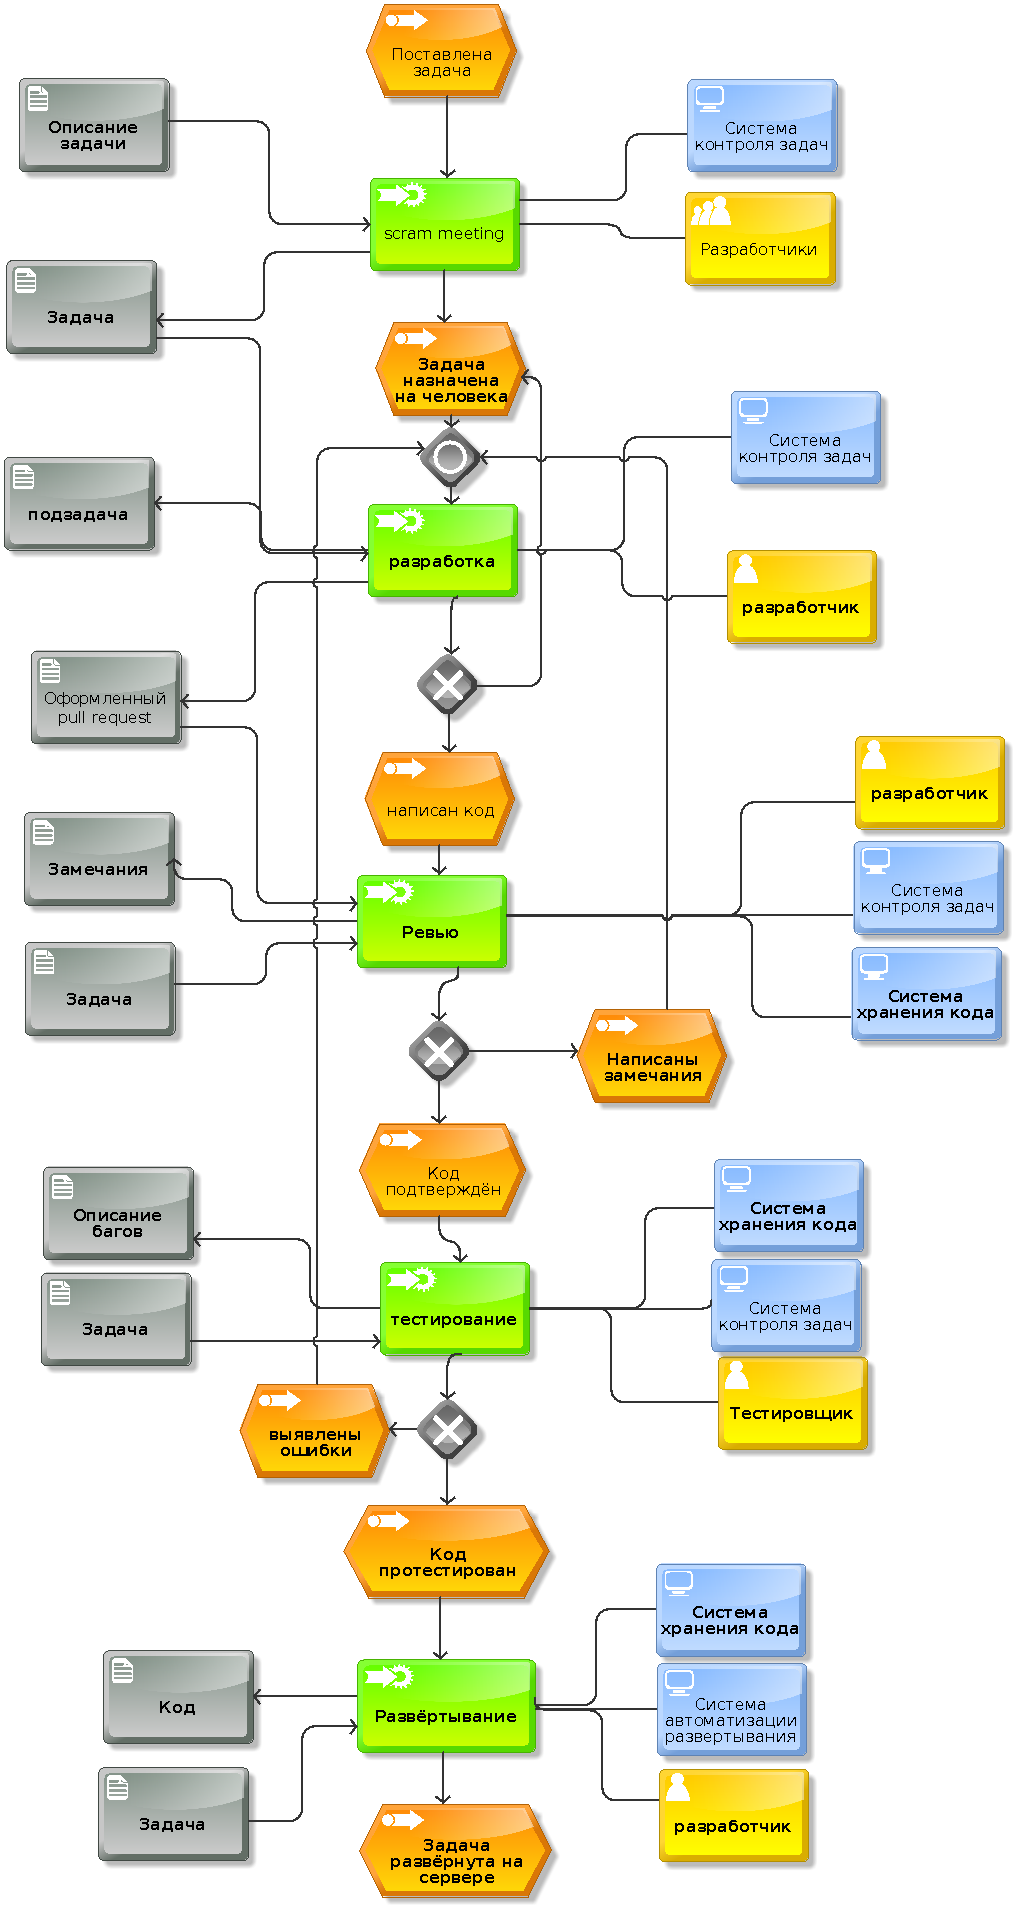
\includegraphics[width=\textwidth]{pictures/2.png}
    \caption{контур разработки}
\end{figure}
\pagebreak
\begin{figure}
    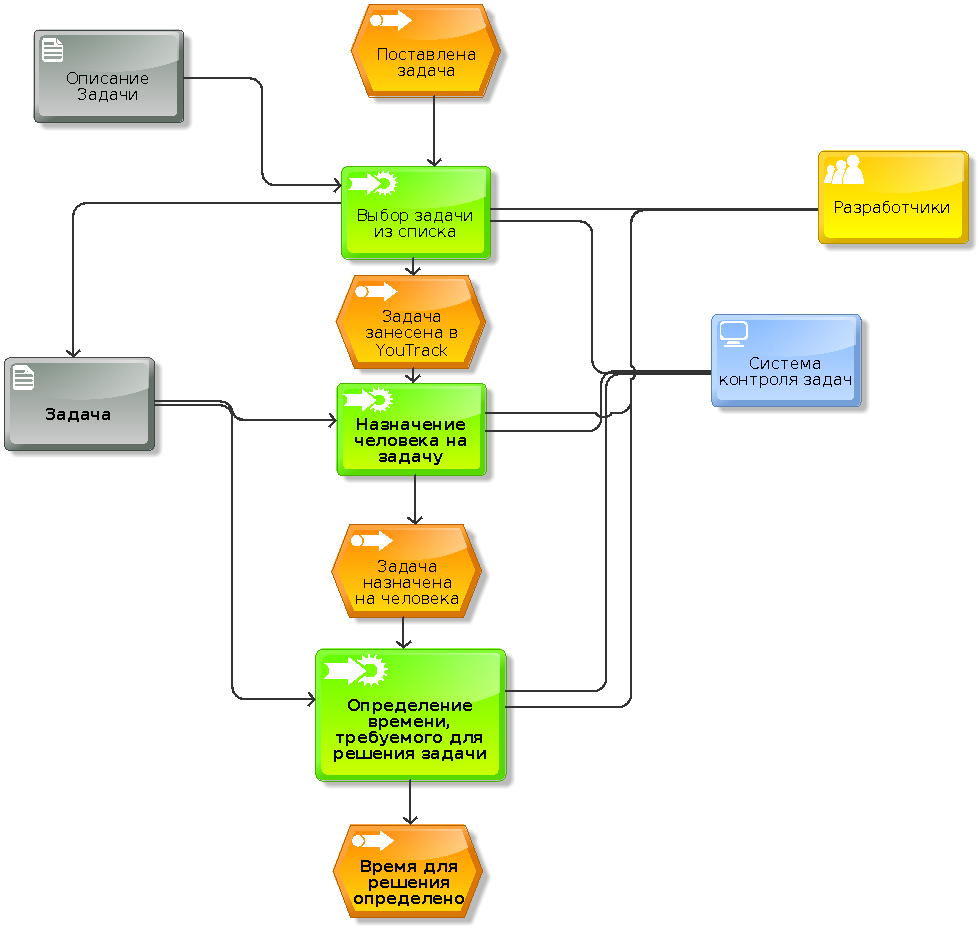
\includegraphics[width=\textwidth]{pictures/3.png}
    \caption{scram meeting}
\end{figure}
\pagebreak
\begin{figure}
    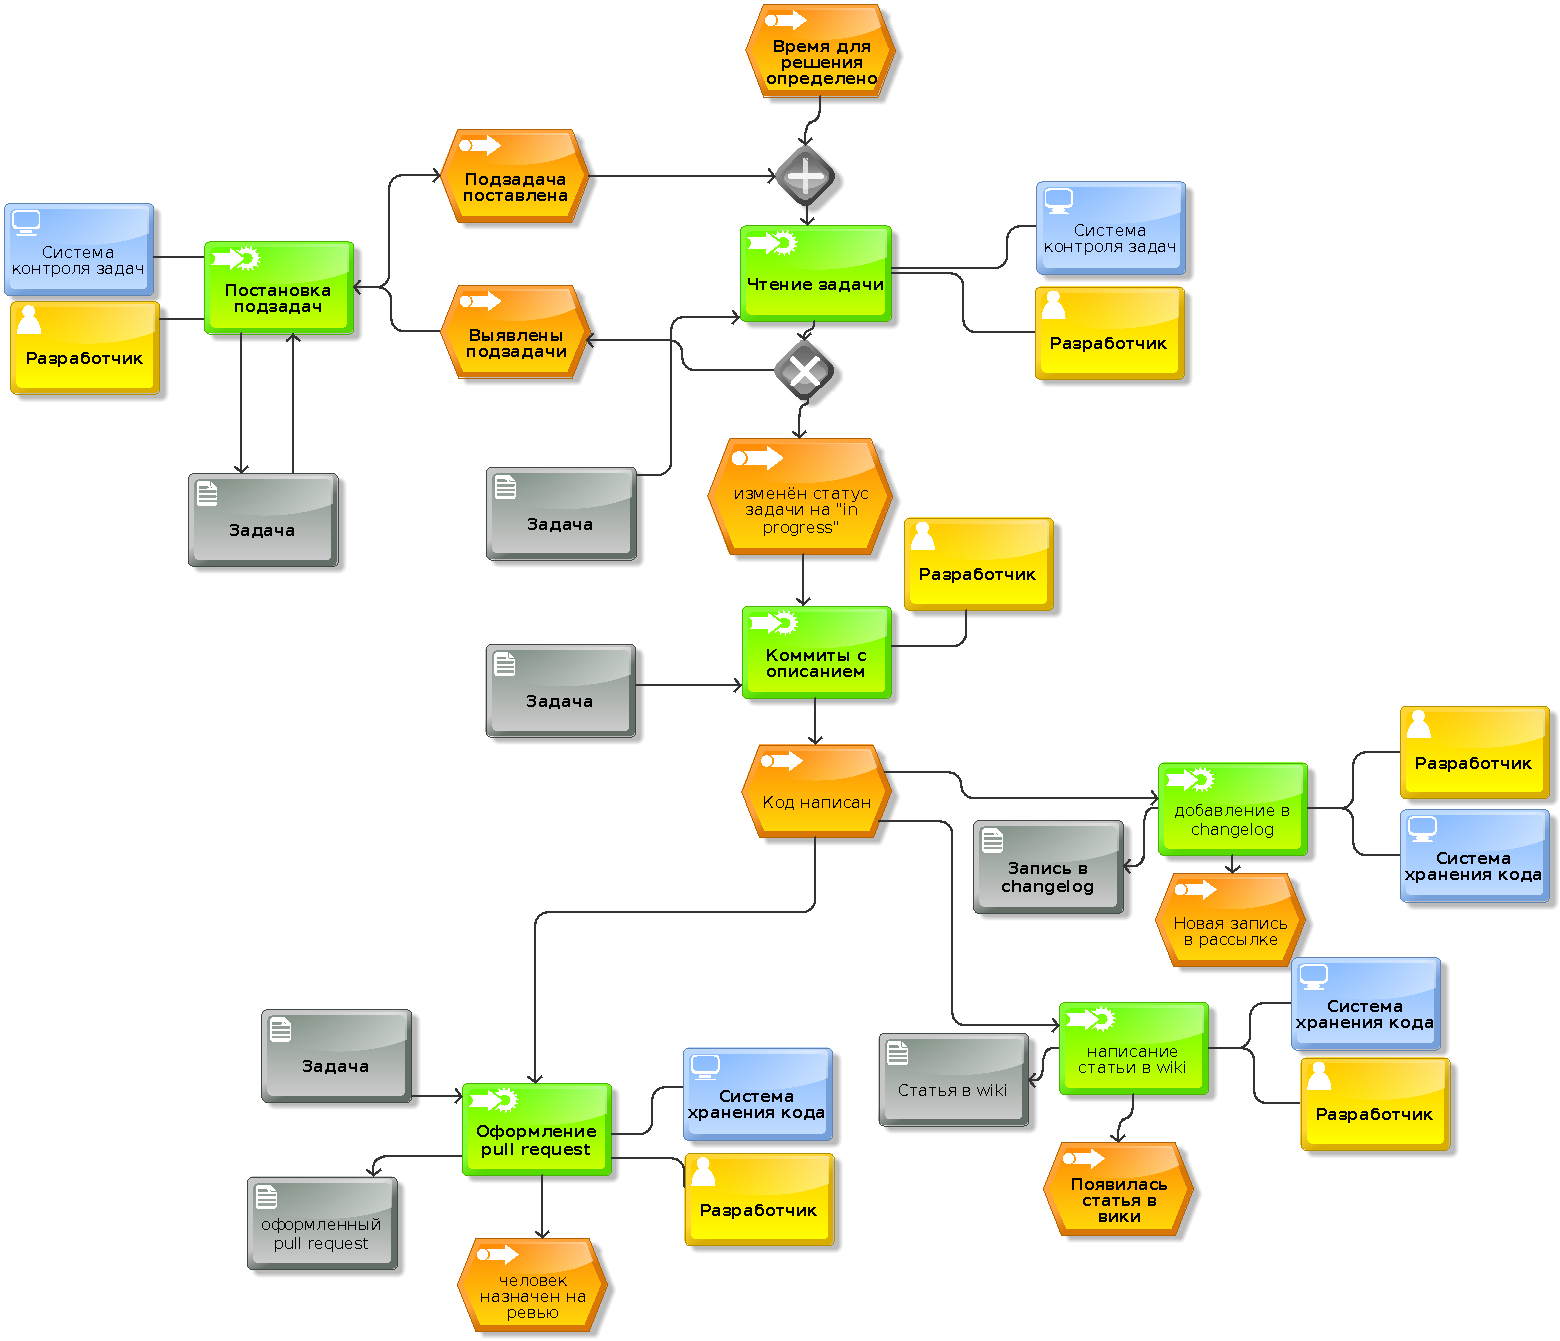
\includegraphics[width=1.2\textwidth]{pictures/4.png}
    \caption{разработка}
\end{figure}
\pagebreak
\begin{figure}
    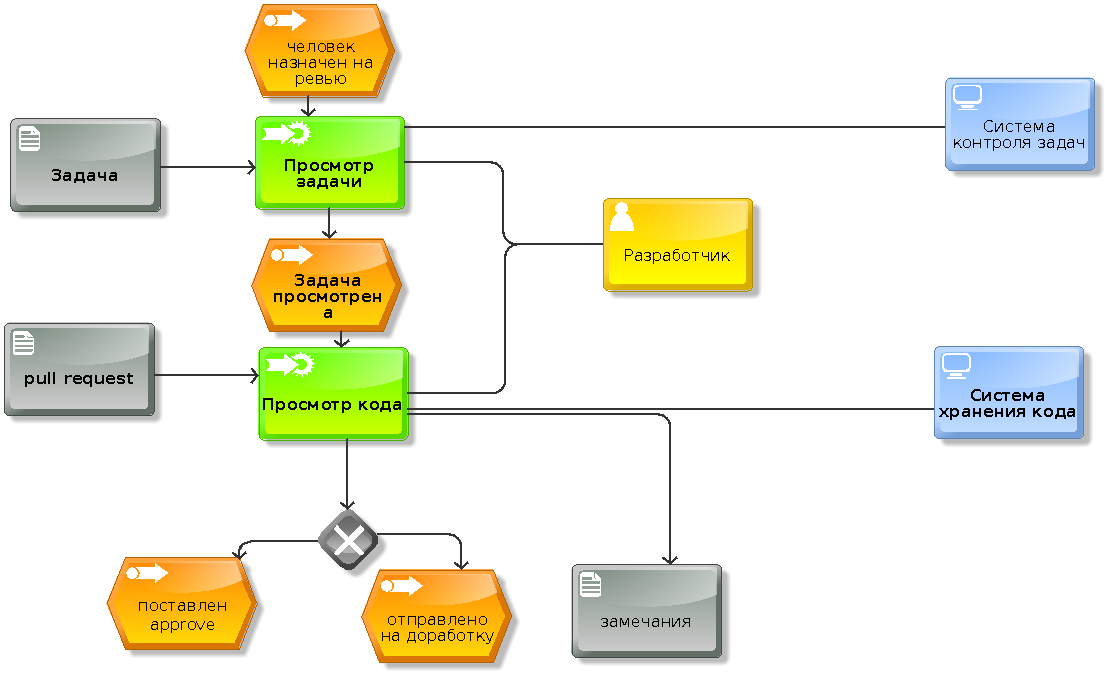
\includegraphics[width=1.2\textwidth]{pictures/5.png}
    \caption{ревью}
\end{figure}
\pagebreak
\begin{figure}
    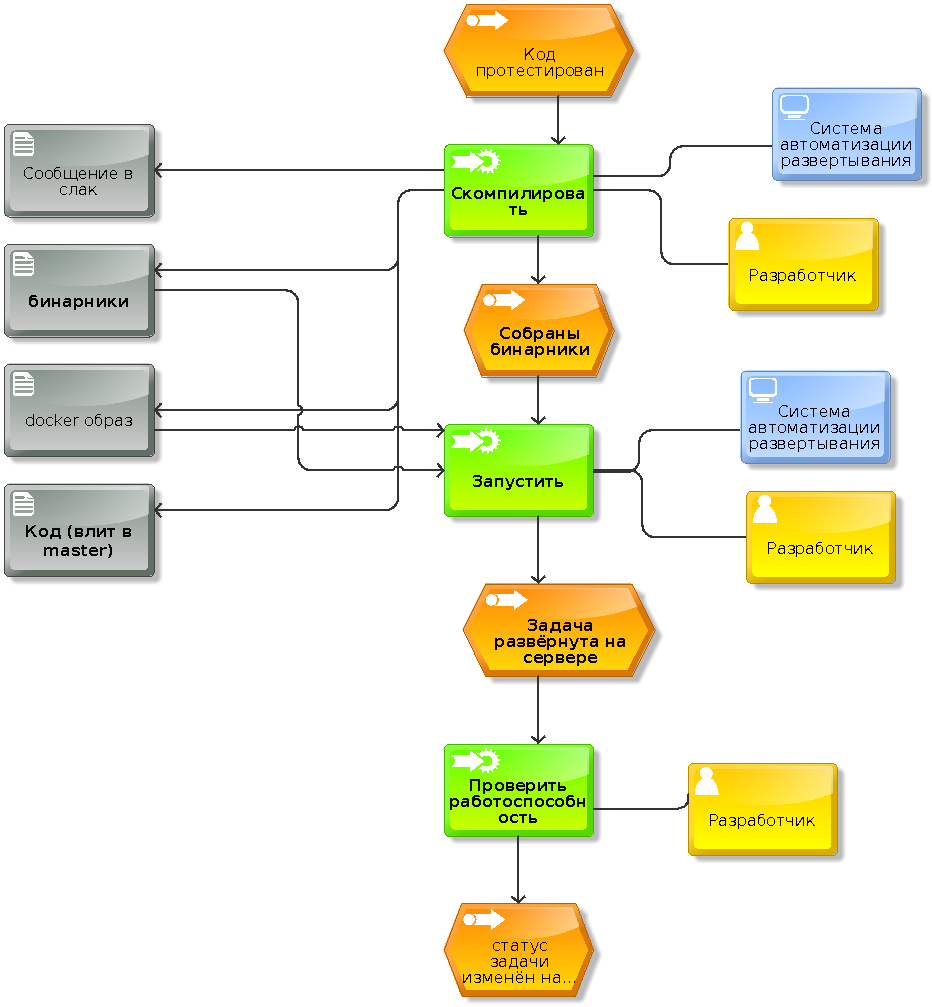
\includegraphics[width=\textwidth]{pictures/7.png}
    \caption{развёртывание}
\end{figure}
\pagebreak

\section{Анализ и моделирование процессов}
% сбор, анализ и
% систематизация информации об объекте автоматизации в рамках выбранной тематики КР,
% моделирование деятельности предприятия, отдельного контура управления предприятием,
% процессов, автоматизируемых выбранным программным средством (средствами),
% формирование требований к средствам автоматизации

% Все процессы можно не брать
% Процессы - это как в первой лабе
% близко рассматривать можно только одну систему
\pagebreak


\section{Анализ средств автоматизации процессов}
% сбор, анализ и
% систематизация информации о средствах автоматизации в рамках выбранной тематики
% КР: функциональных возможностях, реализуемых информационных объектах,
% требованиях к инфраструктуре и способах развертывания, программных компонентах и
% способах их взаимодействия, структурах данных и организации хранилищ данных и т.п.

%   В рамках тематики 2 предполагается структурированное описание
% функциональных возможностей одного или нескольких средств автоматизации,
% применяющихся для автоматизации определенных на предыдущем этапе процессов,
% обоснование возможности их применения (рекомендуется также обосновать выбор
% конкретных средств), сопоставление их функциональных возможностей с требованиями
% процессов, детальное описание требований к ИТ-инфраструктуре со стороны выбранных
% программных средств, рекомендуемых производителем вариантов развертывания этих
% средств и средств их интеграции между собой и с внешними системами.
\pagebreak


\section{Синтез определенных уровней архитектуры ИС}
% (непосредственно проектирование архитектуры ИС на уровне (уровнях), определяемых
% тематикой КР: функциональной архитектуры, информационной архитектуры, системнойархитектуры, программной архитектуры, архитектуры данных, обоснование соответствия
% построенной архитектуры требованиям процессов).

%   В рамках тематики 2 предполагается построение системной архитектуры.
% Необходимо обосновать выбор способа развертывания определенного на предыдущем
% этапе средства автоматизации (или нескольких), включая обоснование количество и
% размещение серверных компонентов, в том числе с использованием технологий
% виртуализации, выбор телекоммуникационных технологий, операционных систем,
% базового программного обеспечения. В описание полученной системной архитектуры
% включаются аппаратные узлы для размещения как серверных, так и клиентских
% компонентов системы, периферийное оборудование, телекоммуникационное
% оборудование, любое системное или вспомогательное программное обеспечение.
% Обосновывается соответствие построенной архитектуры функциональным и
% нефункциональным требованиям, определенным на первом этапе и требованиям к ИТ-
% инфраструктуре со стороны программных средств автоматизации, указанным на втором
% этапе. Указывается за счет каких архитектурных решений обеспечивается требуемый
% уровень производительности (в том числе в условиях изменяющейся нагрузки),
% надежности и безопасности ИС. Описание спроектированной архитектуры
% сопровождается диаграммами, выполненными в соответствии с требованиями нотации
% UML.

\pagebreak


\section{Список использованных источников}

business.radario.ru

приватная вики на гитхабе

\end{document}
